\normaltrue \difficilefalse \tdifficilefalse
\correctionfalse

%\UPSTIidClasse{11} % 11 sup, 12 spé
%\newcommand{\UPSTIidClasse}{12}

\exer{Système bielle manivelle  $\star$ \label{B2:13:12}}
\setcounter{question}{0}\UPSTIcompetence[2]{B2-13}
\index{Compétence B2-13}
\index{Bielle Manivelle}
\index{Moteur}
\ifcorrection
\else
\marginnote{\textbf{Pas de corrigé pour cet exercice.}}
\fi

\ifprof
\else
Soit le mécanisme suivant. On a $\vect{AB}=R\vect{i_1}$ et $\vect{CB}=L\vect{i_2}$. De plus, 
$R=\SI{10}{mm}$ et $L=\SI{20}{mm}$. 

\begin{center}
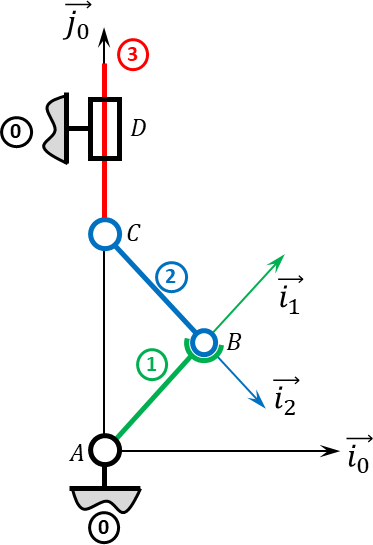
\includegraphics[width=\linewidth]{12_01}
\end{center}
\fi

Il est possible de mettre la loi entrée-sortie sous la forme *** (voir exercice \ref{C2:06:12}).

\question{Donner le torseur cinématique $\torseurcin{V}{2}{0}$ au point $B$.}
\ifprof
\else
\fi

\question{Déterminer $\vectg{C}{2}{0}$.}
\ifprof
\else
\fi


\ifprof
\else
\begin{flushright}
\footnotesize{Corrigé  voir \ref{B2:13:12}.}
\end{flushright}%
\fi